\documentclass{beamer}
\usepackage[utf8]{inputenc}
\usepackage[T1]{fontenc}
\usepackage[french]{babel}
\usepackage{amsmath,amsfonts,amssymb}
\usepackage{graphicx}

\usetheme{Warsaw}

\author{Aurèle Barrière \& Nathan Thomasset}
\title{Cryptographie}
\date{10 mars 2016}


\begin{document}

\begin{frame}
\maketitle
\end{frame}

\begin{frame}{Mise en situation}
  Iseut souhaite envoyer des messages d'amour à Tristan, qui vit en Bretagne avec sa femme. Bien évidemment il ne faut pas que cette dernière puisse les lire, ce qui créerait une situation quelque peu inconfortable.
  \begin{block}{}
   Comment faire pour s'assurer de pouvoir communiquer impunément ?
   \end{block}

  \end{frame}

\begin{frame}{Intérêt de la cryptographie}
  \begin{itemize}
  \item Cartes bleues
    
  \item Mail
    
  \item Transactions bancaires
  
  \item Chiffrement des données sensibles (militaires ou privées)
\end{itemize}
\end{frame}

\begin{frame}{Un codage ultime?}
  Seul quelqu'un qui connaitraît la clé pourrait décoder : est-ce réellement possible ?

Cryptographie symétrique : on a tous les deux une même clé.
\begin{figure}
\centering
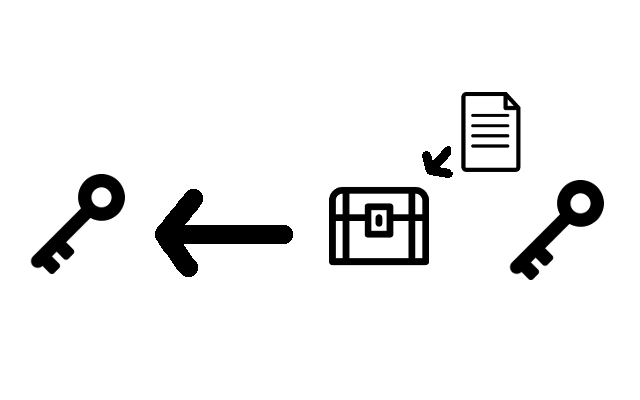
\includegraphics[scale = 0.4]{symetric.png}

\end{figure}
\footnotesize{Source : simpleIcon}
  \end{frame}

\begin{frame}{Exemple : chiffrement de César}
  Décalage constant. 
$$A\rightarrow B, B\rightarrow C, \text{...}$$ 
$$A\rightarrow C, B\rightarrow D, \text{...}$$

  \begin{figure}
    \centering
  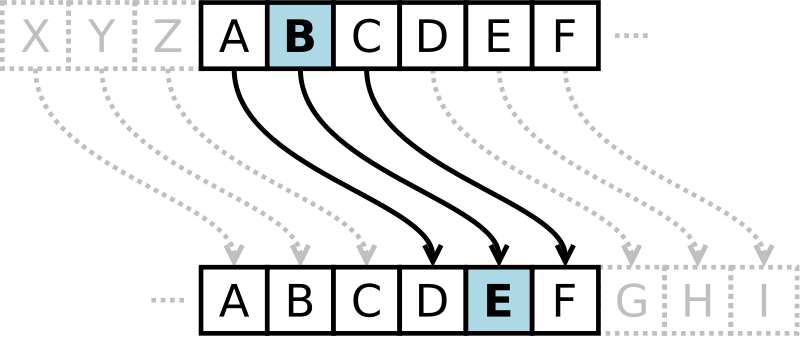
\includegraphics[scale = 0.25]{cesar.png}
\end{figure}
\footnotesize{Source : Wikipedia}
\end{frame}


\begin{frame}{Casser le code de César}
\begin{block}{}
  26 décalages possibles.\\
  Mot à décrypter :  iravivqvqrpelcgv 
\end{block}
  

\footnotesize
\begin{tabular}{c c}
jsbwjwrwrsqfmdhw &  
ktcxkxsxstrgneix\\
ludylytytushofjy &  
mvezmzuzuvtipgkz\\
nwfanavavwujqhla &   
oxgbobwbwxvkrimb\\
pyhcpcxcxywlsjnc & 
qzidqdydyzxmtkod\\
rajerezezaynulpe &
sbkfsfafabzovmqf\\
tclgtgbgbcapwnrg &
udmhuhchcdbqxosh\\
\textbf{\textcolor{red!60!black}{venivididecrypti}} &
wfojwjejefdszquj\\
xgpkxkfkfgetarvk &
yhqlylglghfubswl\\
zirmzmhmhigvctxm &
ajsnaninijhwduyn\\
bktobojojkixevzo &
clupcpkpkljyfwap\\
dmvqdqlqlmkzgxbq &
enwrermrmnlahycr\\
foxsfsnsnombizds &
gpytgtotopncjaet\\
hqzuhupupqodkbfu &
iravivqvqrpelcgv\\
\end{tabular}
\normalsize
  \end{frame}

\begin{frame}{Énumération des clés}
  Énumérer les clés possibles (décalages). Regarder tous les résultats.

  \begin{figure}
    \centering
    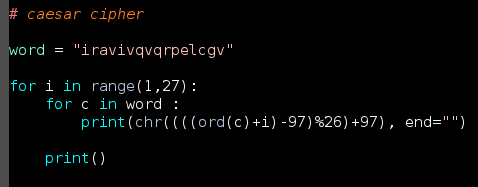
\includegraphics[scale = 0.6]{cesarcode.png}
\end{figure}

\begin{block}{}
Ensemble de clés fini
\end{block}

  \end{frame}



\begin{frame}{Complexité}

  \begin{alertblock}{Le calcul, c'est pas gratuit}
    Trop de clés $\Rightarrow$ trop de calcul, trop de résultats
\end{alertblock}
  L'objectif n'est pas de créer un chiffrement incassable, mais un chiffrement qui soit trop coûteux à casser.

  
  \begin{figure}
  \centering
  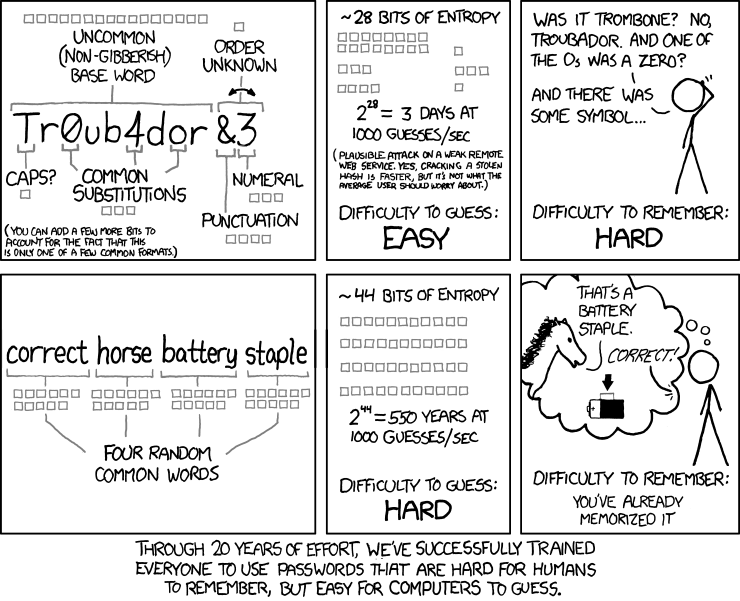
\includegraphics[scale = 0.2]{xkcdpassword_strength.png}
  \end{figure}
\footnotesize{Source : xkcd.com}
  \end{frame}

\begin{frame}{D'autres exemples}
  \begin{block}{Hill}
\centering
    $\begin{pmatrix}
0 & 1 & 0\\
3 & 0 & 2\\
0 & 1 & 1
\end{pmatrix}
\begin{pmatrix}
1\\
2\\
3
\end{pmatrix}
=
\begin{pmatrix}
2\\
9\\
5
\end{pmatrix}$
\end{block}
  \begin{block}{Vigenere}
\centering
\begin{tabular}{ c c c c c c c }
M & E & S & S & A & G & E\\
\hline
C & L & E & C & L & E & C\\
\hline
O & P & W & U & L & K & G
\end{tabular}
\end{block}
  \end{frame}

\begin{frame}{Analyse fréquentielle}
  \begin{alertblock}{Trop de clés}
    Matrices 3$\times$3 : 5429503678976
    
    Matrices 10$\times$10 : \\
314293064158293883017435778850162642728266998876247525637
417317539899590842010402346543259906970228933096407508161
1719197835869803511992549376
    \end{alertblock}

\begin{figure}
\centering
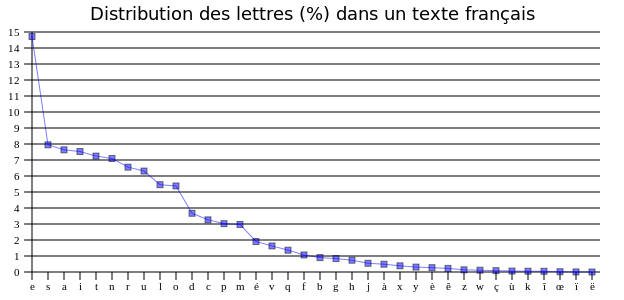
\includegraphics[scale = 0.38]{distribution.png}
\end{figure}
\footnotesize{Source : manudiclemente, Wikipedia}
  \end{frame}


\begin{frame}{Cryptographie asymétrique}
  Tristan a perdu la clé. Ne pouvant pas la faire refaire, il leur faut trouver un nouveau moyen de communiquer.
      \end{frame}

\begin{frame}{RSA}
    \begin{figure}
    \centering
    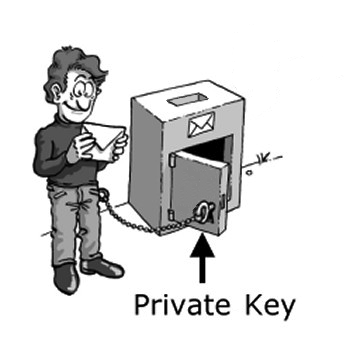
\includegraphics[scale = 0.5]{Public_Key.png}
  \end{figure}
  \end{frame}

\begin{frame}{Limites}
  \begin{figure}
    \centering
    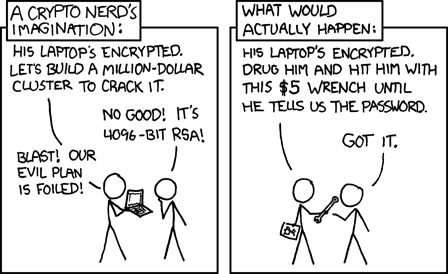
\includegraphics[scale = 0.5]{xkcdsecurity.png}
  \end{figure}
\footnotesize{Source : xkcd.com}
\end{frame}

\begin{frame}{Conclusion}
  \begin{center}
  Cryptographie symétrique et asymétrique

  Énumération des clés  

  Complexité du calcul
\end{center}

  
  GPG mail

  \end{frame}





\end{document}
